\documentclass[12pt]{article}
\usepackage{float}
\usepackage{graphicx}
\usepackage{tabularx}
\usepackage[font=small,labelfont=bf]{caption}
\usepackage{xcolor}
\usepackage{hyperref}

\pagestyle{empty}
\setcounter{tocdepth}{4}
\setcounter{secnumdepth}{4}

\topmargin=0cm
\oddsidemargin=0cm
\textheight=22.0cm
\textwidth=16cm
\parindent=0cm
\parskip=0.15cm
\topskip=0truecm
\raggedbottom
\abovedisplayskip=3mm
\belowdisplayskip=3mm
\abovedisplayshortskip=0mm
\belowdisplayshortskip=2mm
\normalbaselineskip=12pt
\normalbaselines

\begin{document}

\vspace*{0.5in}
\centerline{\bf\Large Iteration 3 - Test Document}

\vspace*{0.5in}
\centerline{\bf\Large Team PA-PI-a}

\vspace*{0.5in}
\centerline{\bf\Large 8 April 2018}

\vspace*{1.5in}
\begin{table}[htbp]
\caption{Team}
\begin{center}
\begin{tabular}{|r | c|}
\hline
Name & ID Number \\
\hline\hline
Melanie Taing & 40009850 \\
Laurie Gagnon & 22943433 \\
Wayne Yiel Leung & 26586988 \\
Jordan Rutty & 27300107 \\
Michael Foo & 40000225 \\
Pierre-Andre Leger & 40004010 \\
Colin Greczkowski & 40001600 \\
\hline
\end{tabular}
\end{center}
\end{table}

\clearpage

\pagenumbering{roman}
\pagestyle{plain}

\tableofcontents
\clearpage

\listoffigures
\newpage

\pagenumbering{arabic}
\pagestyle{plain}

\section{Introduction}
The purpose of this document is to gather all information necessary for testing of the MyMoney application. This document describes the testing approach and overall framework that will be used to test the MyMoney application.\\

The following pages will identify the requirements that will be tested, the testing strategy used, the test cases and their results, and the description of input files.

\section{Test Plan}

{\it
Describe what forms of testing you plan to do (unit, subsystem, integration),
describe briefly the schedule and resources for testing,
and
how you designed your test cases.

Indicate which qualities (from requirements) were tested and which qualities were not tested.
}

\subsection{System Level Test Cases}
{\it
All test cases for testing at the system level.}

\noindent
{\bf Purpose}\\
State the purpose of the test.
Indicate which requirement and which aspect of that requirement is being tested.

\noindent
{\bf Input Specification}\\
State the context for the test in terms of system state.
State the input test data. You may need to mention operations invoked as well as data for the operation.
You can cross-reference to actual file data specified in an appendix.

\noindent
{\bf Expected Output}\\
State the expected system response and output.
You can cross-reference to actual file data specified in an appendix.

\noindent
{\bf Traces to Use Cases}\\
State which requirements (at the level of use case and scenario) are tested by this test case.
\clearpage

% Test case 6.1
\subsubsection{Test Case 6.1} \label{6.1}

\noindent
{\bf Purpose}\\
The purpose of the test is to verify the user is able to add a bank account into the application's database.
It satisfies the requirement of the user being able to create a bank account.

\noindent
    {\bf Input Specification}\\
    The application displays a graphical user interface on the screen.
    Optionally, it shows a list of pre-existing bank accounts in the window's top-right corner.
    MyMoney accepts any kind of characters and of any length as input in the \textit{Bank} and \textit{Nickname} fields while
    the \textit{Balance} field accepts non-negative integers. The \textit{Bank} and \textit{Balance} fields cannot be empty.
    The user presses \textit{Add} on the interface to add the account.
    
\noindent
    {\bf Expected Output}\\
    The application displays the window.
    A created bank account with the information the user entered now exists in the application.
    
\noindent
    {\bf Traces to Use Cases}\\
    This test case satisfies the main scenario of use case 1 - \textit{AddAccount}.

% Test case 6.2
\subsubsection{Test Case 6.2} \label{6.2}
\noindent
{\bf Purpose}\\
        The test verifies that for an existing bank account its bank name, nickname and balance can be modified.
        This satisfies the requirement that the user is able to adjust account information in case of an account transfer
        to another financial institution. 

\noindent
{\bf Input Specification}\\
            MyMoney displays a graphical user interface on the screen.
            For this operation, MyMoney accepts any kind of characters and of any length as
            input in the \textit{Bank} and \textit{Nickname} fields while the \textit{Balance} field accepts non-negative integers.
            The \textit{Bank} and \textit{Balance} fields cannot be empty. The user presses the \textit{Update} to update the account information.
            
\noindent
{\bf Expected Output}\\
    The application displays the window.    
    The system displays updated information of the bank account in the top-right window.

 \noindent
 {\bf Traces to Use Cases}\\
     This satisfies the main scenario of use case 2 - \textit{UpdateAccount}.
                    

%Test case 6.3
\clearpage %%%%%%%%%%%%%CAN BE REMOVED IF THE TEST CASE DISPLAYS ON SINGLE PAGE
\subsubsection{Test Case 6.3} \label{6.3}
\noindent
{\bf Purpose}\\
 This test verifies the user is able to delete their own account.
 This satisfies the requirement that the user is able to remove their account when their is no longer associated
 with a bank. 

 \noindent
 {\bf Input Specification}\\
 MyMoney displays a graphical user interface on the screen.
 For this operation, the user selects their account with the mouse and presses \textit{Delete}.
                            
 \noindent
 {\bf Expected Output}\\
 The application displays the window.
 Also it display a list of accounts in the top-right corner except the one that was deleted.

\noindent
{\bf Traces to Use Cases}\\
This satisfies the main scenario of use case 3 - \textit{DeleteAccount}.


%Test case 6.4
\subsubsection{Test Case 6.4} \label{6.4}

\noindent
{\bf Purpose}\\
This test verifies the user is able to add a transaction into their existing account.
This satisfies the requirement that the user can complete an addition of a transaction into their account.
                                        
\noindent
{\bf Input Specification}\\
MyMoney displays a graphical user interface on the screen.
For this operation, MyMoney accepts a transaction \textit{type} - withdraw or deposit, a \textit{date}
which is selected via the date picker, an \textit{Amount}, a integer, a \textit{Budget} which is chosen
from a drop-down list, and a \textit{description} - a string composed of any characters and
of non-negative length. To register the action, the user presses \textit{Add} located in the bottom left
of the window.                                          

\noindent
{\bf Expected Output}\\
The application displays the window.    
The transaction is added to the account.
If the user selects his account in the top-right corner of the window then
the bottom-right window displays the newly created transaction.
                                                
\noindent
{\bf Traces to Use Cases}\\
This satisfies the main scenario of use case 4 - \textit{AddTransaction}.


%Test case 6.5
\clearpage %%%%%%%%%%%%%CAN BE REMOVED IF THE TEST CASE DISPLAYS ON SINGLE PAGE
\subsubsection{Test Case 6.5} \label{6.5}

\noindent
{\bf Purpose}\\
This test verifies the user is able to import a transaction into their existing account.
This satisfies the requirement that the user can import a transaction into their account.
                                                        

\noindent
{\bf Input Specification}\\
MyMoney displays a graphical user interface on the screen.
For this operation, the user selects their account with the mouse,
clicks the import button, chose the csv file.
                                                          

\noindent
{\bf Expected Output}\\
The transaction is added to the user's account.
The bottom-right corner displays the transaction.


\noindent
{\bf Traces to Use Cases}\\
This satisfies use case 5 - \textit{ImportTransactions}



%Test case 6.6
\subsubsection{Test Case 6.6} \label{6.6}
\noindent
{\bf Purpose}\\
This test verifies the user is able to update an existing transaction in their account.
This satisfies the requirement that the user can change information of a transaction in their account.
                                                        

\noindent
{\bf Input Specification}\\
MyMoney displays a graphical user interface on the screen.
For this operation, the user selects their account with the mouse,
chose the appropriate transaction to modify in the bottom-right window.
The user can modify the transaction fields on the transactions pane.
In the pane, transaction \textit{type} - withdraw or deposit, a \textit{date}
which is selected via the date picker, an \textit{Amount}, a integer, a \textit{Budget} which is chosen
from a drop-down list, and a \textit{description} - a string composed of any characters and
of non-negative length. The register the action, the user presses \textit{Add} located in the bottom left
of the window.   
                                                          

\noindent
{\bf Expected Output}\\
The application displays the window.    
The fields in the transaction are updated.
If selected, the bottom-right corner displays the updated transaction.

\noindent
    {\bf Traces to Use Cases}\\
    This satisfies use case 6 - \textit{ImportTransactions}

%Test case 6.7
\clearpage %%%%%%%%%%%%%CAN BE REMOVED IF THE TEST CASE DISPLAYS ON SINGLE PAGE
\subsubsection{Test Case 6.7} \label{6.7}
\noindent
{\bf Purpose}\\
This test verifies the user is able to delete an existing transaction in their account.
This satisfies the requirement that the user can changeremove a transaction from their account.
                                                        
\noindent
{\bf Input Specification}\\
MyMoney displays a graphical user interface on the screen.
For this operation, the user selects their account with the mouse,
chose the appropriate transaction to remove in the bottom-right window.
The user presses \textit{Delete} in the Transactions pane.
                                                          

\noindent
{\bf Expected Output}\\
The application displays the window.       
The transaction does not show in the bottom-right window.

\noindent
{\bf Traces to Use Cases}\\
This satisfies use case 7 - \textit{DeleteTransactions}

\def\arraystretch{1.5}%
\begin{table}[htbp]
\centering
\caption{Template Test Case}
\label{UT-1}
\begin{tabularx}{\textwidth}{ | l | X |}
\hline
\textbf{Test Case Number}      &  UT-1                         \\ \hline
\textbf{Test Case Description}    &  This test case is used to ensure the generated puzzle board has the same dimensions as the input width and height                \\ \hline
\textbf{Input}         & 	\begin{enumerate}
	\item None - Default 8-8 board size
	\item  Width/height from "input.txt" file. 
\end{enumerate} \\ \hline

\textbf{Expected Output}     & \begin{enumerate}
	\item "OK" - Test executed successfully.
\end{enumerate} \\ \hline
\textbf{Expected Post-Conditions}           &  The system responds to the presence or absence of the input vector and outputs a success message upon test successful completion in "output.txt", along with a time-stamp containing the test's execution time and date.                    \\ \hline
\textbf{Execution History}   &  \begin{enumerate}
	\item 05/04/2018 | Tester's name | Executed test successfully.
\end {enumerate} \\ \hline
\end{tabularx}
\end{table}
\clearpage


\subsection{Subsystem Level Test Cases}

{\it
All test cases for testing at the subsystem level.
}

{\it
One subsection per subsystem
}

\subsubsection{Subsystem X}

\subsection{Unit Test cases}

{\it
All test cases for testing at the unit level.
}

{\it
One subsection per unit
}


\subsubsection{Unit Test Case 1} \label{tc:1}
\def\arraystretch{1.5}%
\begin{table}[htbp]
\centering
\caption {UT-1}
\label{UT-1}
\begin{tabularx}{\textwidth}{ | l | X |}
\hline
\textbf{Test Case Number}      &  UT-1                         \\ \hline
\textbf{Test Case Description}    &  This test case is used to ensure that transactions are properly saved or updated to their repository                \\ \hline
\textbf{Input}         & 	\begin{enumerate}
	\item A Transaction object populated with generic data
          \item A second Transaction object with the ID of the first one.
	\item A test transaction database.
\end{enumerate} \\ \hline

\textbf{Expected Output}     & \begin{enumerate}
	\item Transaction details are printed to console.
\end{enumerate} \\ \hline
\textbf{Expected Post-Conditions}           &  A transaction database is created and a transaction is inserted. The balance of this transaction is then updated to a new value.                   \\ \hline
\textbf{Execution History}   &  \begin{enumerate}
	\item 04/03/2018 | Colin Greczkowski | Executed test successfully.
\end {enumerate} \\ \hline
\end{tabularx}
\end{table}
\clearpage

\subsubsection{Unit Test Case 2} \label{tc:2}
\def\arraystretch{1.5}%
\begin{table}[htbp]
\centering
\caption {UT-2}
\label{UT-2}
\begin{tabularx}{\textwidth}{ | l | X |}
\hline
\textbf{Test Case Number}      &  UT-2                         \\ \hline
\textbf{Test Case Description}    &  This test verifies that the deleteItem method works as intended, and deletes a Transaction record for a given ID                \\ \hline
\textbf{Input}         & 	\begin{enumerate}
          \item A generic account ID
	\item A Transaction object populated with generic data, associated to the generic account.
	\item A test transaction database.
\end{enumerate} \\ \hline

\textbf{Expected Output}     & \begin{enumerate}
	\item "Delete Transaction 1"
\end{enumerate} \\ \hline
\textbf{Expected Post-Conditions}           & The test transaction database should be empty.                \\ \hline
\textbf{Execution History}   &  \begin{enumerate}
	\item 04/07/2018 | Colin Greczkowski | Executed test successfully.
\end {enumerate} \\ \hline
\end{tabularx}
\end{table}
\clearpage

\subsubsection{Unit Test Case 3} \label{tc:3}
\def\arraystretch{1.5}%
\begin{table}[htbp]
\centering
\caption {UT-3}
\label{UT-3}
\begin{tabularx}{\textwidth}{ | l | X |}
\hline
\textbf{Test Case Number}      &  UT-3                         \\ \hline
\textbf{Test Case Description}    &  This test case is used to make sure all Transactions associated to an account are properly purged from the repository.                \\ \hline
\textbf{Input}         & 	\begin{enumerate}
          \item A generic account ID
	\item Two Transaction objects populated with generic data, associated to the generic account.
	\item A test transaction database.
\end{enumerate} \\ \hline

\textbf{Expected Output}     & \begin{enumerate}
	\item "Delete Transaction 1"
           \item "Delete Transaction 2"
\end{enumerate} \\ \hline
\textbf{Expected Post-Conditions}           & The test transaction database does not contain the two transactions that had the generic account ID.                \\ \hline
\textbf{Execution History}   &  \begin{enumerate}
	\item 04/03/2018 | Colin Greczkowski | Executed test successfully.
\end {enumerate} \\ \hline
\end{tabularx}
\end{table}
\clearpage

\subsubsection{Unit Test Case 4} \label{tc:1}
\def\arraystretch{1.5}%
\begin{table}[htbp]
\centering
\caption {UT-4}
\label{UT-4}
\begin{tabularx}{\textwidth}{ | l | X |}
\hline
\textbf{Test Case Number}      &  UT-4                         \\ \hline
\textbf{Test Case Description}    &  This tests the RepositoryContainer's ability to save a variety of types of objects (Transactions, Accounts, Budgets).                \\ \hline
\textbf{Input}         & 	\begin{enumerate}
          \item Test Transaction, Budget and Account Databases
	\item A test Transaction
	\item A test Account
	\item A test Budget
\end{enumerate} \\ \hline

\textbf{Expected Output}     & \begin{enumerate}
	\item The test transaction's details are printed to console.
\end{enumerate} \\ \hline
\textbf{Expected Post-Conditions}           & The account,transaction and budget items are saved to their respective test databases. Balances are updated correctly.                \\ \hline
\textbf{Execution History}   &  \begin{enumerate}
	\item 04/07/2018 | Colin Greczkowski | Executed test successfully.
\end {enumerate} \\ \hline
\end{tabularx}
\end{table}
\clearpage


\subsubsection{Unit Test Case 5} \label{tc:1}
\def\arraystretch{1.5}%
\begin{table}[htbp]
\centering
\caption {UT-5}
\label{UT-5}
\begin{tabularx}{\textwidth}{ | l | X |}
\hline
\textbf{Test Case Number}      &  UT-5                         \\ \hline
\textbf{Test Case Description}    &  TO BE COMPLETED: BudgetContainer test                \\ \hline
\textbf{Input}         & 	\begin{enumerate}
	\item A Budget object populated with generic data
	\item A test Account database with transactions
	\item A test Budget database
\end{enumerate} \\ \hline

\textbf{Expected Output}     & \begin{enumerate}
	\item The test budget's details are printed to console.
\end{enumerate} \\ \hline
\textbf{Expected Post-Conditions}           & A budget database is created and a budget is inserted. The recorded budget amount is updated according to transactions made across all accounts for that budget.            \\ \hline
\textbf{Execution History}   &  \begin{enumerate}
	\item 04/08/2018 | Melanie Taing | Not executed
\end {enumerate} \\ \hline
\end{tabularx}
\end{table}
\clearpage



%Account repository test case
\begin{table}[htbp]
\centering
\label{UT-6}
\begin{tabularx}{\textwidth}{ | l | X |}
\hline
\textbf{Test Case Number}      &  UT-6                      \\ \hline
\textbf{Test Case Description}    &  This test case is used to ensure created accounts are saved in the database. Also it verifies that accounts can be deleted from it.                 \\ \hline
\textbf{Input}         & 	\begin{enumerate}
  
\item An account database
\item An account repository
\item An account with non-null values for \textit{nickname}, \textit{bankName} and a non-negative value for \textit{balance}
  
\end{enumerate} \\ \hline

\textbf{Expected Output}     & \begin{enumerate}
\item Tuples in Account repository test before delete: 2 
\item Tuples in Account repository test after delete: 1 
\item Current items loaded in repo:1 
\item 1

\end{enumerate} \\ \hline
\textbf{Expected Post-Conditions} & The system has a single account in the account database. \\
\hline
\textbf{Execution History}   &  \begin{enumerate}
	\item 04/07/2018 | Wayne Yiel Leung | Executed test failed.
\end {enumerate} \\ \hline
\end{tabularx}
\end{table}




\section{Test Results}

{\it
List the tests, indicating which passed and which did not pass.
List requirements indicating the percentage of tests that passed for that requirement.
}

\section{References}

\section{Addendum}

\begin{figure}[H]
\centering
\caption{Updated use case diagram}
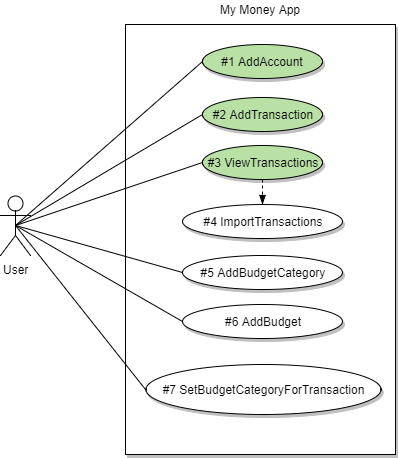
\includegraphics[scale=0.5]{Diagrams/UML/SOEN.png}
\end{figure}

\section{Description of Input Files}

Describe/include test data from input files.

\end{document}
